\subsection{Sprachübertragung}

\subsubsection*{Übersicht}



\subsubsection*{Benutzeroberfläche}

Button Screen wie IP5 \\
Active Call Screen \\
Erweiterte Inbox \\
Neue Screens für Gegensprechanlage. \\
Erweiterung Admin UI für Konfiguration CallType \\


\subsubsection*{Konfiguration}
Erweiterung Configuration Domain um CallType.
Hat text property, dass als Anzeige auf dem Button dient.
Hat Liste von Clients, die im Call angesprochen werden können.


\subsubsection*{Verfügbarkeit und Registrierung}

Client muss sich beim Startup beim Signaling Service registrieren.

\subsubsection*{Verbindungsaufbau}

\begin{figure}[h]
    \centering
    \begin{minipage}[b]{0.9\textwidth}
        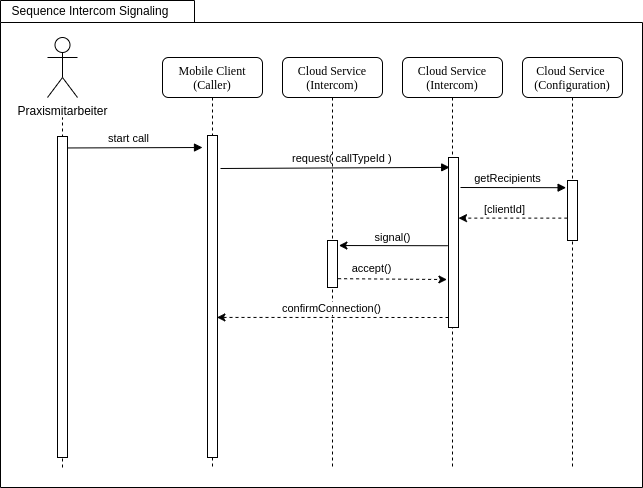
\includegraphics[width=\textwidth]{graphics/diagramms/Sequence_Intercom_Broking_V01}
        \caption{Ablauf Verbindungsaufbau Gegensprechanalge}
    \end{minipage}
\end{figure}



\subsubsection*{Unterhaltung}

Mute Button
End Call Button


\subsubsection*{Verbindungsende}

Caller nimmt Finger vom Button.
Receiver hat button zum abbrechen.



\subsection{Übersicht Erweiterung Praxisruf Cloud Service}

\begin{figure}[h]
    \centering
    \begin{minipage}[b]{0.9\textwidth}
        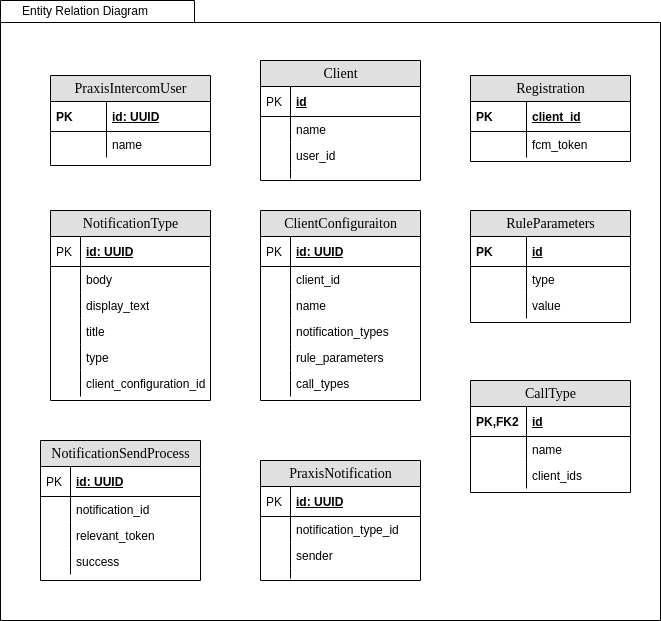
\includegraphics[width=\textwidth]{graphics/diagramms/erd_v01}
        \caption{Ablauf Verbindungsaufbau Gegensprechanalge}
    \end{minipage}
\end{figure}



\clearpage
